\hyperref[sec:sec24]{\section{為什麼外國政府常常對香港問題說三道四?}}
\label{sec:sec17}

首先,香港政制本身要求香港政府邀請其他國家就香港事務發表意見。《基本法》第三十九條規定「《公民權利和政治權利國際公約》、《經濟、社會與文化權利的國際公約》和國際勞工公約適用於香港的有關規定繼續有效,通過香港特別行政區的法律予以實施。」特區成立以來,政府多次向聯合國提交報告交待香港的人權狀況,並派員出席人權事務委員會的會議,回答委員的質詢。過去的質詢,包括盡快實現普選、外籍家傭工被虐待的問題,和少數族裔的教育問題等。香港的民間團體也會列席相關的聯合國會議。簡單來說,外國政府對香港的問題發表意見,其實是《基本法》得到落實的體現。

拉闊一點去想,從全球化的框架下思考國際關係,儘管中國政府經常宣稱香港事務屬中國內政,但站在外國政府的立場來說,他們如何和香港打交道也是他們的內政。由於他們設定對港政策之前,必須先對中國大陸和香港的關係作出獨立的評估,因此他們關心香港的具體情況,也是正常的政府行為。

香港能成為一個特區,很大程度上要外國政府的認同才能有實際意義。畢竟,特區的特別之處,往往關乎涉外事務。舉個例,北韓也可以把境內某個地方劃為特區,但如果外國不認為這個地方和北韓的其他地方有什麼現實上的分別,不對這個地方作出任何差別對待,這個所謂的「特區」就會變成一紙虛文。

放在香港,儘管《基本法》容許香港單獨與各國簽署雙邊協定,但對方是否願意和香港簽署這些協定,卻是該等國家的主權範圍。例如說香港相對於中國大陸是一個獨立的關稅區,和擁有獨立入境的地位,都並不是中國政府自己宣稱便會有效。有些外國政府會對香港出產的貨品提供免稅優惠,對中國大陸出產的卻不會;有些外國政府會對香港特區護照持有人提供免簽證待遇,對中國護照的持有人卻不會。這些差異都是建基於他們相信香港特區和中國大陸之間有現實上的區隔。如果有天中國大陸的貨品可以隨便在香港換上香港製造的標籤,中國護照的持有人可以隨便在香港拿到特區護照,而香港政府又無從阻擋的話,那麼外國政府就很有可能會撤銷對香港的差別待遇,香港作為一個特區的實際意義就會大幅下降。

以美國的《美國—香港政策法》(又稱《香港關係法》)為例,就規定於一九九七年七月一日之後,如總統斷定香港已沒有足夠的自主性以獲得某些美國法律的差別待遇,則可以行政命令暫定該等法律在香港適用。舉個例,美國有一些科技產品是可以出口到香港而不可以出口到中國大陸的,如果美國發現出口到香港和出口到中國大陸已沒有差別,當然會停止對香港出口這些產品。

美國奉行三權分立,為確保聯邦政府有切實執行《香港關係法》,國務院會不時向國會提交報告,介紹港美關係和香港有否嚴格落實高度自治。這些報告的內容包括和美國直接相關的部分,例如當香港於二零一七年首次拒絕把一名美國的通輯犯移交美國,反而按中國政府的要求將之移交中國大陸,而中國大陸方面卻沒有公佈相關案件的處理情況。報告中也會論及香港的整體情況,例如眾多媒體被於中國大陸有商業利益的公司控制,新聞從業員認為它們會因經濟和政治原因作自我審查等。

為調查實況,美國國會也會邀請香港的政治領袖出席作證,讓美國的民意代表更有效監督聯邦政府對《香港關係法》的實施,儘管這些聽證會在中國政府的眼中就是香港的反對派到外國抹黑中國。站在中國政府的立場來說,香港有多少自主是中國內政,美國無權過問;但在美國政府的立場來說,美國如何對待香港是美國政府的工作,而這點基於美國認為香港有多少自主,所以有責任主動搞清楚。而如果有天美國真的要撤除對香港的差別待遇,也會對美國自身的利益會帶來一定衝擊,因此美國見到可導致此事發生的發展時向中國和香港政府作出提醒,正常不過。

\begin{figure}[htbp]
    \centering
    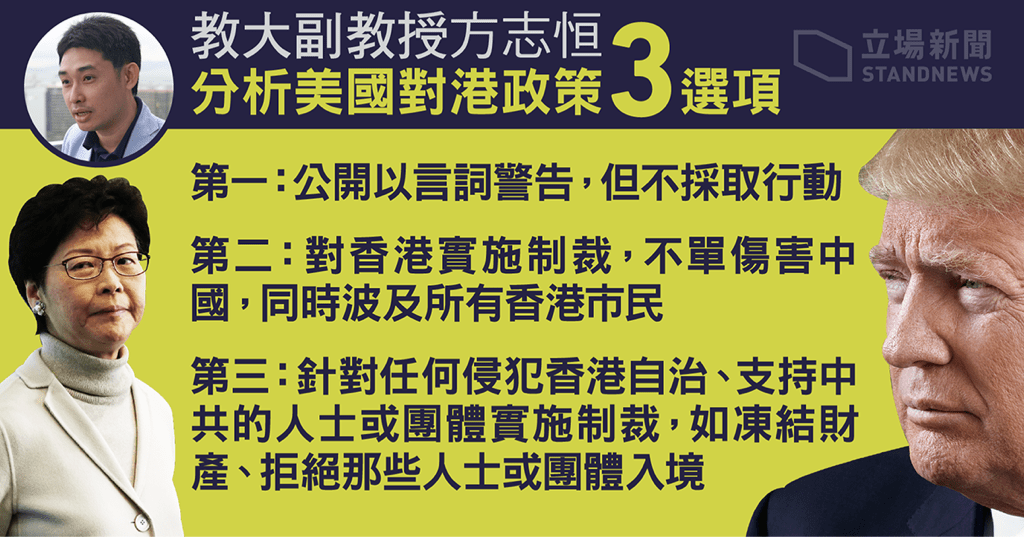
\includegraphics[width=0.7\textwidth]{c17/h-klesson1-024.png}
    \caption{《香港政策法》成為香港近年熱議題目} 
\end{figure}

說到底,活在全球化的年代,已沒有一個地方可以不和其他地方打交道。所謂拒絕「干預內政」的說法其實是一把雙面刃,世界各地可以同一板斧來回應中國。例如香港政府在中國政府的壓力下可阻礙台灣政界甚至學界前來香港交流,又可拒絕為外國駐港記者續期簽證,並且不予任何解釋;但對方同樣可以為香港特區護照持有人的入境增添困難而不予任何理由。如果香港的學生即使獲哈佛或耶魯取錄卻因拿不到學生簽證而不能入境,又或對香港出口美國的貨品被徵收與中國同等的稅項,雖然理論上也是美國政府的內部決定,卻肯定會引起香港市民對香港和中國政府的不滿。

相對於其他國家政府對香港的關注,英國政府的關注則更難稱為說三道四。英國政府外交大臣自一九九七年七月一日起每半年向英國國會提交有關《中英聯合聲明》在港實施情況的報告。中國外交部發言人曾聲言《聯合聲明》是一份歷史文件,不具有任何現實意義,英國政府以此為基礎評論香港事務並無根據。現實來說《聯合聲明》的功能當然沒有因為香港特區的成立和《基本法》的實施而終止,因為《基本法》本身就引述了《聯合聲明》作為規範。

《中英聯合聲明》的其中一項主要內容,是就中國對香港的「基本方針政策」作出說明,其中附件一就是以「中華人民共和國政府對香港的基本方針政策的具體說明」為題。站在中國政府的立場來說,《聯合聲明》第三條第十二項提到這些「基本方針政策」和其具體說明將會「以中華人民共和國香港特別行政區基本法規定之」,那麼既然《基本法》已經生效,《聯合聲明》是否就完成了其歷史任務?翻開《基本法》第一百五十九條,列明「本法的任何修改,均不得同中華人民共和國對香港既定的基本方針政策相抵觸」,而《基本法》的前言又提到「國家對香港的基本方針政策,已由中國政府在中英聯合聲明中予以闡明」。換言之,《基本法》是不可以隨意修改的,任何對《基本法》的修改均不能違反《聯合聲明》中所說明的「基本方針政策」。由是觀之,只要《基本法》繼續存在,《聯合聲明》都有實際上的意義(起碼直至所載的「基本方針政策」在二零四七年到期為止,見\hyperref[sec:sec36]{問題三十六})。

當然,條文文本是一件事,實際操作又是另一件事。假若有日出現疑似違反《中英聯合聲明》的《基本法》修正案,香港人可否拿去終審法院按第一百五十九條的規定覆核是否合憲?就算到時法院願意受理,又會否出現新一輪的人大釋法把第一百五十九條或前言的相關字眼解釋一次?到時終審法院可以怎麼辦呢(見\hyperref[sec:sec25]{問題二十五})?這些執行上的問題,就要回到中國《憲法》中對特區的地位無甚保障的現實去談(見\hyperref[sec:sec16]{問題十六})。


回到外國政府對香港「說三道四」的批評,香港既為國際城市,香港涉外事務本身就是一個大題目,足以引起外國關注的情況數之不盡。例如近年有不少外國政府關注香港的企業或團體是否成為了中國的「白手套」,通過遊說、商業活動,甚至非法行為協助中國在外國達到各種經濟及政治目的,如自然資源開採和港口投資等(何志平案就是一例)。又或香港本身相對中立的國際地位,會否為中國所用影響國際政治,如曾任香港衛生署署長的陳馮富珍在中國政府的推舉下成為世界衛生組織總幹事。凡此種種,當中國政府越排距外國政府對香港的關注,長遠來說恐怕越會打擊香港在國際社會中的地位,對中國政府來說也未必是一件好事。而所謂的外部勢力,也不應理解為鐵板一塊,不同國家有不同盤算,同一國家內政治菁英、商界、學者,以至民間社會也可有不同盤算,即使對香港的管治提出質疑也可理由各異;把這些統統視為非黑即白的敵我矛盾,等於幫助對手團結起來,減少自己可能的盟友,同樣非常不智。

\rule[-10pt]{15cm}{0.05em}

伸延閱讀:

Postiglione GA and Yang JTH (ed) (1997) \textit{Hong Kong’s Reunion with China: The Global Dimensions, New York: ME Sharpe}.

Shen S (2016) \textit{Hong Kong in the World: Implications to Geopolitics and Competitiveness}, London: Imperial College Press.

網上資源:

\href{https://thestandnews.com/politics/分析美國對港政策-3-選項-方志恒-美國可制裁侵犯香港自治人士-凍結資產拒入境/}{立場報道(2019):〈分析美國對港政策 3 選項 方志恒:美國可制裁侵犯香港自治人士 凍結資產拒入境〉:立場新聞,2019年5月17日}